\section{Smart Contract: ExamContract}

Per la realizzazione dello smart contract, è stata utilizzata la piattaforma Ethereum. In particolare, il contratto è stato scritto in Solidity, il linguaggio di programmazione orientato agli oggetti, più diffuso per l'implementazione di contratti intelligenti su varie piattaforme blockchain tra cui Ethereum stessa. In fine, il contratto è stato deployato sulla rete di test Goerli, in quanto Ropsten risulta deprecata dal 21 Gennaio e verrà disabilitata nel Q4 del 2022.\\
\\
Durante l'analisi dei requisiti, ci si è resi conto che nonostante l'utilizzo dell'indirizzo garantisca pseudo-anonimicità, non è particolarmente user-friendly. Per questo, si è deciso di utilizzare un'associazione tra indirizzo pubblico e matricola, permettendo l'utilizzo di quest'ultima per l'inserimento di voti da parte del prof.\\
\\
Nella fase di progettazione, si è deciso di separare il sorgente in due file diversi. Nel primo file, IExamContract.sol, è stata definita l'interfaccia del contratto, definendo metodi, strutture ed eventi. Questa scelta ha permesso di individuare tutte le funzionalità da implementare prima di definirne dettagli. Successivamente, è stato realizzato ExamContract.sol, un'implementazione dell'interfaccia discussa sopra.

\subsection{Controlli sulle dipendenze}
Per rendere più completo il contratto, è stata aggiunta la possibilità di definire propedeuticità a livello di materie e dipendenze tra test della stessa materia. Dall'analisi dei requisiti, sono stati individuati diversi scenari.
Per quanto riguarda le materie, non sono state rilevate grandi difficoltà.
Una materia può avere delle propedeuticità, ma una volta superate la materia è disponibile per il resto della carriera universitaria.
Prendendo in esempio la propedeuticità:
$$
    Prog1 \rightarrow Prog2
$$
E' possibile definire all'interno di Prog1 una lista di materie che verranno `Sbloccate' al superamento. Per stabilire se una materia è sbloccata o meno, è stato utilizzato un contatore, inizializzato con il numero di materie propedeutiche.
\pagebreak\\
\\
Con questa soluzione, internamente si avrà:
\begin{minted}{python}
prog1 = {counter: 0, unlocks: [prog2]}
prog2 = {counter: 1, unlocks: []}
# Superamento esame di prog1 per lo studente stud1
for unlock in prog1.unlocks:
    stud1.materia(unlock).counter -=1
\end{minted}



\subsection{Tipologie di utenti}
\label{sec:roles}
Sempre durante la fase di progettazione, sono state identificate tre tipologie di utenti:
\begin{itemize}
    \item Admin
    \item Professore
    \item Studente
\end{itemize}

\subsubsection{Admin}
La prima tipologia di utente, corrisponde al creatore del contratto. Quest'ultimo ha la possibilità di definire il nome, le propedeuticità e i relativi CFU delle materie, l'associazione tra matricola ed indirizzo pubblico e la gestione della lista dei professori autorizzati alla verbalizzazione dei test e del voto finale delle singole materie. In generale, è possibile considerare questo account come la componente amministrativa dell'università, per questo motivo ci riferiremo a questo ruolo con il termine `University' nelle figure successive.

\subsubsection{Professore}
Nonostante abbia la capacità di definire le caratteristiche della materie, la definizione dei test spetta alla seconda tipologia di utente, il professore.
Quest'ultimo, dopo aver ricevuto l'autorizzazione da parte dell'admin, può invocare la funzione \texttt{setSubjectTests()}, passando una lista di oggetti \texttt{Test} che verrà discussa successivamente. In \autoref{fig:create_subject} è possibile vedere il diagramma di flusso, con tutti gli attori coinvolti.\\
\\
Il professore ha inoltre la possibilità di proporre un voto finale, tramite la funzione \texttt{setSubjectResults()}, specificando come argomento una lista di coppie \texttt{<Matricola,VotoFinale>}. Il voto finale dovrà essere esplicitamente accettato dallo studente, come descritto in \autoref{fig:registerSubjectVotes}

\begin{figure}
    \centering
    \includegraphics[width=0.70\columnwidth]{img/CreateSubject.png}
    \caption{Diagramma di flusso: `Create a subject'}
    \label{fig:create_subject}
\end{figure}

\begin{figure}
    \centering
    \includegraphics[width=0.85\columnwidth]{img/SubjectVote.png}
    \caption{Diagramma di flusso: `Register subject votes'}
    \label{fig:registerSubjectVotes}
\end{figure}

\pagebreak

\subsubsection{Studente}
L'ultima tipologia di utente progettata è lo studente. E' identificato da una matricola univoca e dal relativo indirizzo pubblico. Affinché un utente venga riconosciuto dal contratto come studente, è necessario che esista l'associazione $\textit{Indirizzo pubblico} \Rightarrow \textit{Matricola}$, aggiunta precedentemente dall'admin.
Sostanzialmente lo studente ha accesso a tre funzioni:
\begin{itemize}
    \item Rifiutare il voto di un test
    \item Accettare/Rifiutare la proposta di voto di una materia
    \item Resettare tutti i test di una materia
\end{itemize}



\begin{figure}
    \centering
    \includegraphics[width=0.75\columnwidth]{img/TestVote.png}
    \caption{Diagramma di flusso: `Register test votes'}
    \label{fig:registerTestVotes}
\end{figure}


\begin{figure}
    \centering
    \includegraphics[width=0.75\columnwidth]{img/TestGraph.png}
    \caption{Schema delle prove}
    \label{fig:testGraph}
\end{figure}

%\resizebox{!}{\textheight}{
    \definecolor{plantucolor0000}{RGB}{255,255,255}
    \definecolor{plantucolor0001}{RGB}{0,0,0}
    \definecolor{plantucolor0002}{RGB}{255,255,255}
    \definecolor{plantucolor0003}{RGB}{24,24,24}
    \definecolor{plantucolor0004}{RGB}{255,192,203}
    \definecolor{plantucolor0005}{RGB}{173,216,230}
    \definecolor{plantucolor0006}{RGB}{144,238,144}
    \definecolor{plantucolor0007}{RGB}{226,226,240}
    \definecolor{plantucolor0008}{RGB}{254,255,221}
    \definecolor{plantucolor0009}{RGB}{238,238,238}
    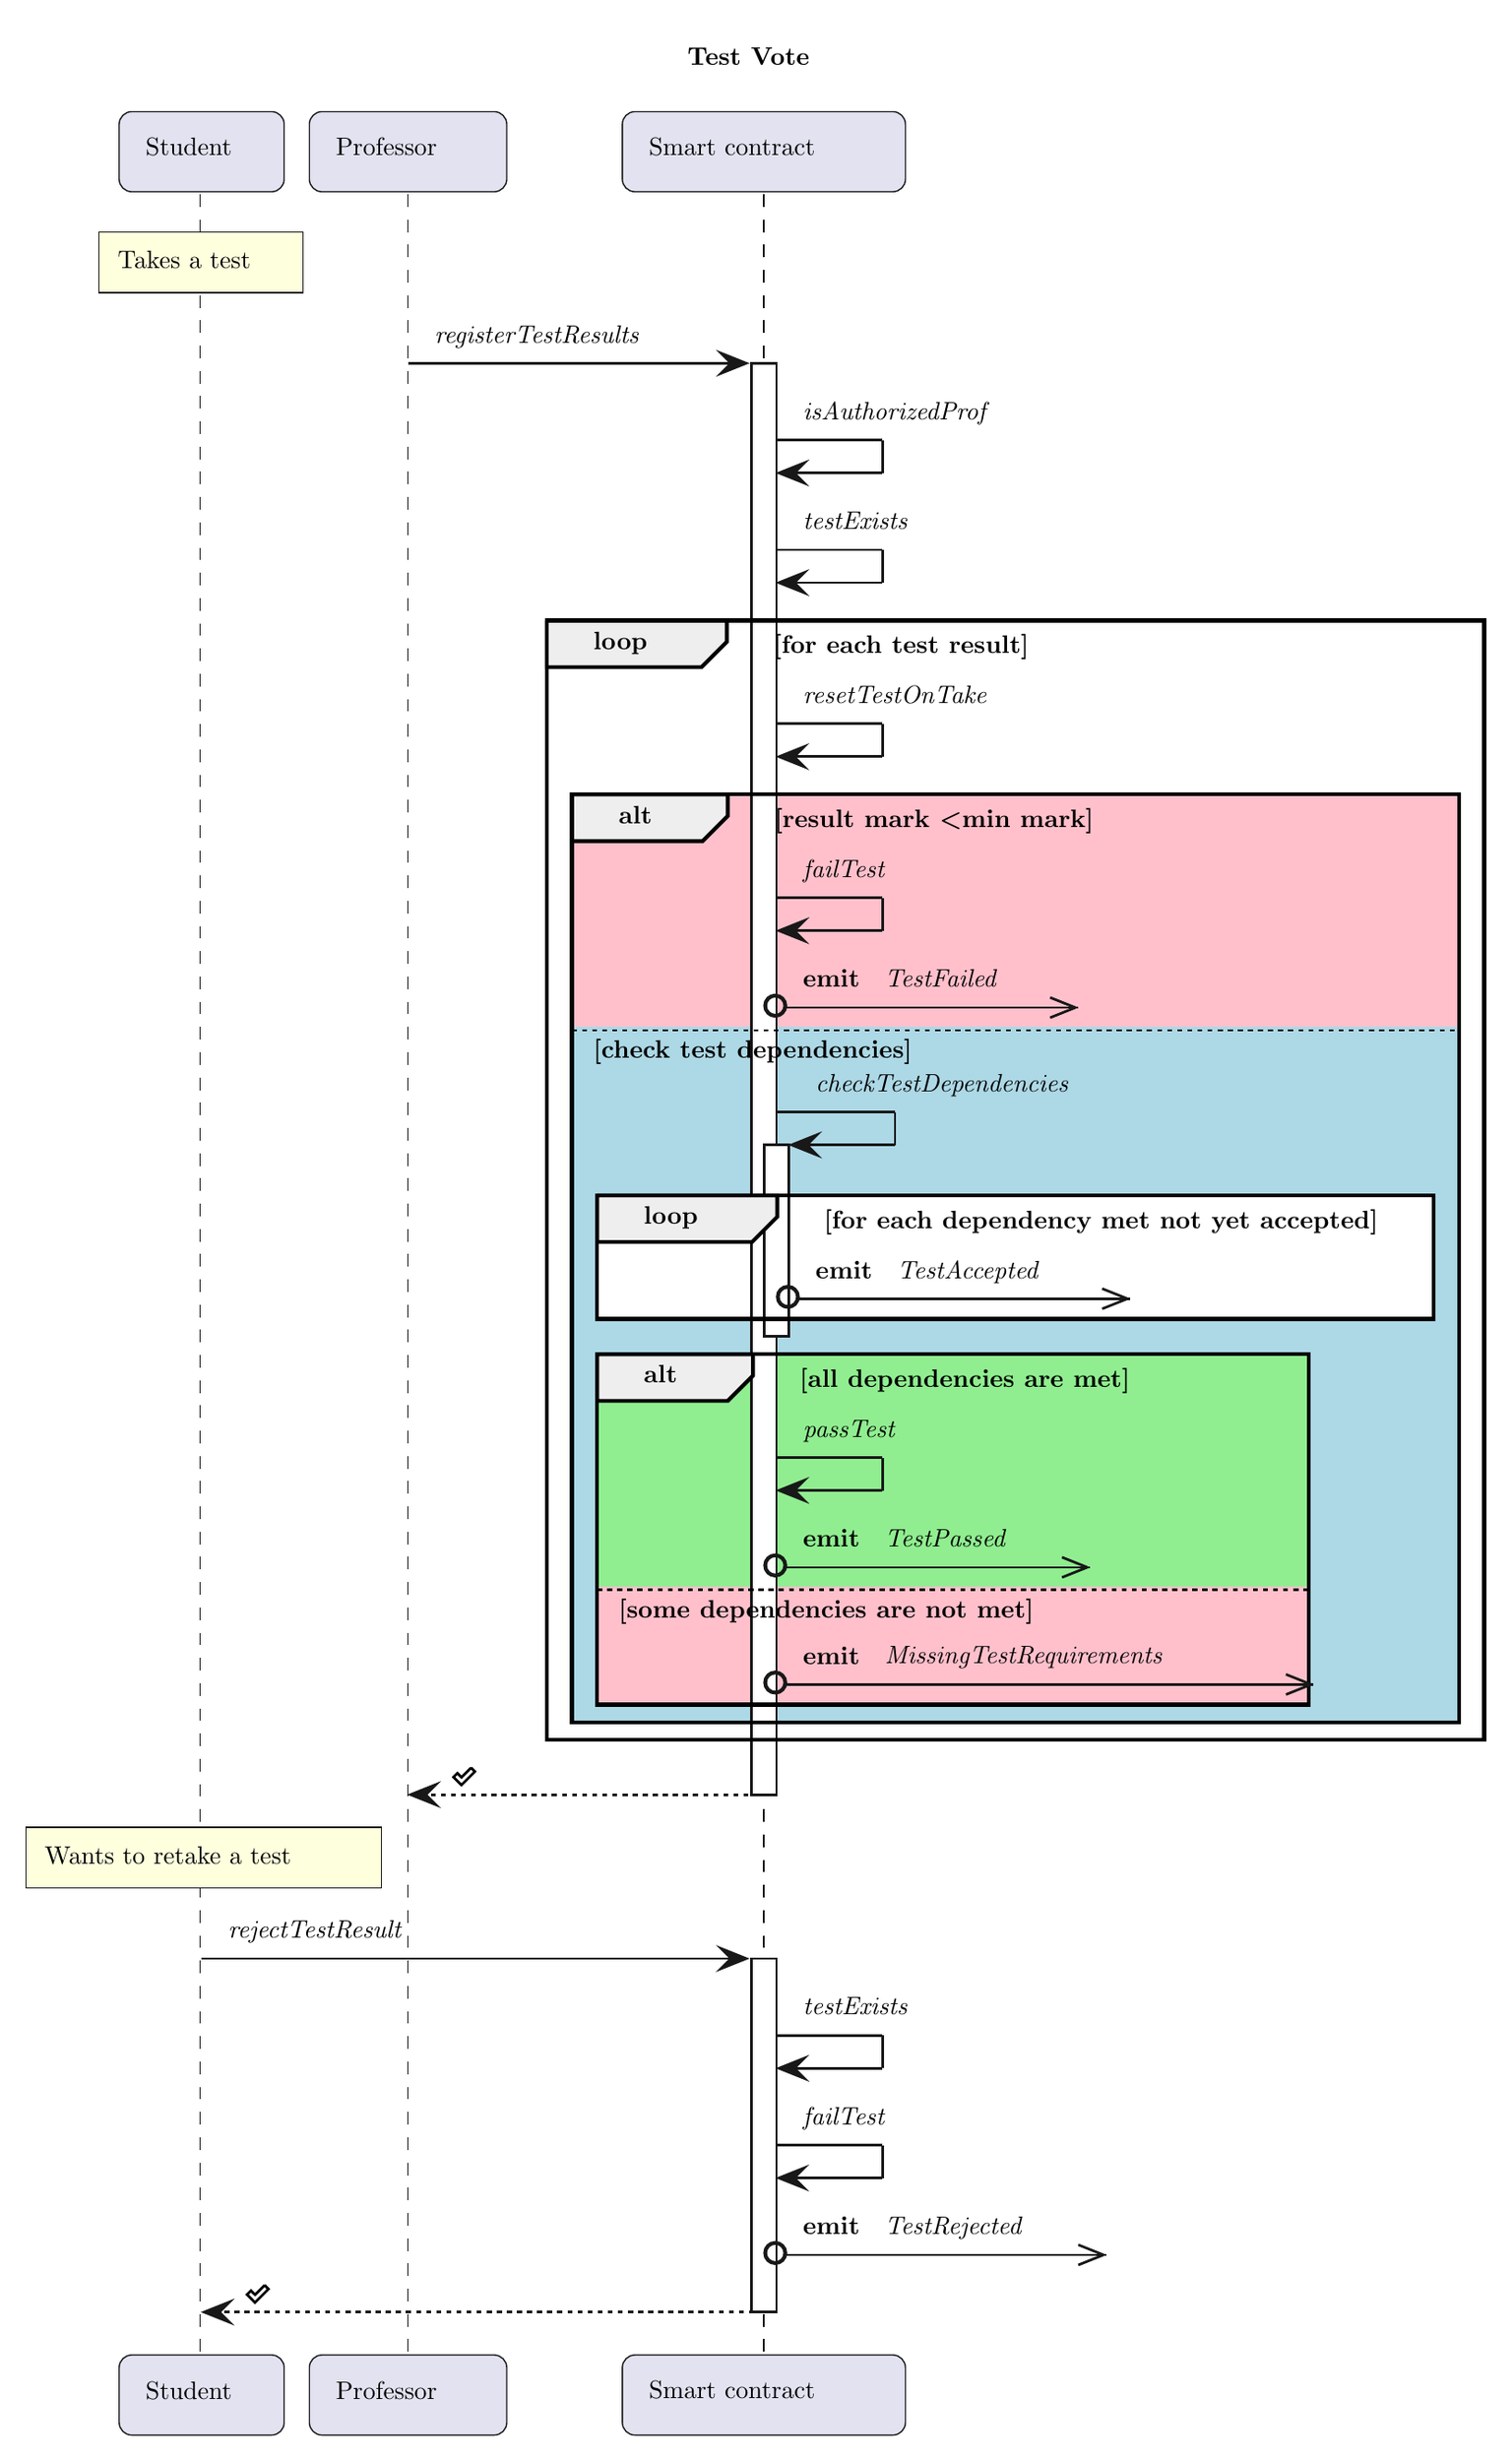
\begin{tikzpicture}[yscale=-1
            ,pstyle1/.style={color=plantucolor0003,fill=white,line width=1.0pt}
            ,pstyle2/.style={color=black,line width=1.5pt}
            ,pstyle8/.style={color=plantucolor0003,line width=0.5pt,dash pattern=on 5.0pt off 5.0pt}
            ,pstyle9/.style={color=plantucolor0003,fill=plantucolor0007,line width=0.5pt}
            ,pstyle10/.style={color=plantucolor0003,fill=plantucolor0008,line width=0.5pt}
            ,pstyle11/.style={color=plantucolor0003,fill=plantucolor0003,line width=1.0pt}
            ,pstyle12/.style={color=plantucolor0003,line width=1.0pt}
            ,pstyle13/.style={color=black,fill=plantucolor0009,line width=1.5pt}
            ,pstyle14/.style={color=plantucolor0003,line width=1.5pt}
            ,pstyle15/.style={color=black,line width=1.0pt,dash pattern=on 2.0pt off 2.0pt}
            ,pstyle16/.style={color=plantucolor0003,line width=1.0pt,dash pattern=on 2.0pt off 2.0pt}
            ,pstyle17/.style={color=black,line width=1.0pt}
        ]
        \draw[color=plantucolor0000,line width=1.0pt] (258.7931pt,10pt) rectangle (333.4237pt,37.7461pt);
        \node at (263.7931pt,15pt)[below right,color=black]{\textbf{Test Vote}};
        \draw[pstyle1] (292.617pt,143.4492pt) rectangle (302.617pt,710.7018pt);
        \draw[pstyle1] (297.617pt,453.2207pt) rectangle (307.617pt,529.1777pt);
        \draw[pstyle1] (292.617pt,775.6589pt) rectangle (302.617pt,915.7611pt);
        \draw[pstyle2] (211.4993pt,245.4063pt) rectangle (583.2168pt,689.0352pt);
        \draw[color=black,fill=plantucolor0004,line width=1.5pt] (221.4993pt,314.3633pt) rectangle (573.2168pt,682.0352pt);
        \draw[fill=plantucolor0005,color=plantucolor0005,line width=1.0pt] (221.4993pt,406.7988pt) rectangle (573.2168pt,682.0352pt);
        \draw[color=black,fill=white,line width=1.5pt] (231.4993pt,473.2207pt) rectangle (563.2168pt,522.1777pt);
        \draw[color=black,fill=plantucolor0006,line width=1.5pt] (231.4993pt,536.1777pt) rectangle (513.6083pt,675.0352pt);
        \draw[fill=plantucolor0004,color=plantucolor0004,line width=1.0pt] (231.4993pt,628.6133pt) rectangle (513.6083pt,675.0352pt);
        \draw[pstyle8] (74pt,76.4922pt) -- (74pt,933.7611pt);
        \draw[pstyle8] (156.414pt,76.4922pt) -- (156.414pt,933.7611pt);
        \draw[pstyle8] (297.4993pt,76.4922pt) -- (297.4993pt,933.7611pt);
        \draw[pstyle9] (42pt,48.7461pt) arc (180:270:5pt) -- (47pt,43.7461pt) -- (102.414pt,43.7461pt) arc (270:360:5pt) -- (107.414pt,48.7461pt) -- (107.414pt,70.4922pt) arc (0:90:5pt) -- (102.414pt,75.4922pt) -- (47pt,75.4922pt) arc (90:180:5pt) -- (42pt,70.4922pt) -- cycle;
        \node at (49pt,50.7461pt)[below right,color=black]{Student};
        \draw[pstyle9] (42pt,937.7611pt) arc (180:270:5pt) -- (47pt,932.7611pt) -- (102.414pt,932.7611pt) arc (270:360:5pt) -- (107.414pt,937.7611pt) -- (107.414pt,959.5072pt) arc (0:90:5pt) -- (102.414pt,964.5072pt) -- (47pt,964.5072pt) arc (90:180:5pt) -- (42pt,959.5072pt) -- cycle;
        \node at (49pt,939.7611pt)[below right,color=black]{Student};
        \draw[pstyle9] (117.414pt,48.7461pt) arc (180:270:5pt) -- (122.414pt,43.7461pt) -- (190.6685pt,43.7461pt) arc (270:360:5pt) -- (195.6685pt,48.7461pt) -- (195.6685pt,70.4922pt) arc (0:90:5pt) -- (190.6685pt,75.4922pt) -- (122.414pt,75.4922pt) arc (90:180:5pt) -- (117.414pt,70.4922pt) -- cycle;
        \node at (124.414pt,50.7461pt)[below right,color=black]{Professor};
        \draw[pstyle9] (117.414pt,937.7611pt) arc (180:270:5pt) -- (122.414pt,932.7611pt) -- (190.6685pt,932.7611pt) arc (270:360:5pt) -- (195.6685pt,937.7611pt) -- (195.6685pt,959.5072pt) arc (0:90:5pt) -- (190.6685pt,964.5072pt) -- (122.414pt,964.5072pt) arc (90:180:5pt) -- (117.414pt,959.5072pt) -- cycle;
        \node at (124.414pt,939.7611pt)[below right,color=black]{Professor};
        \draw[pstyle9] (241.4993pt,48.7461pt) arc (180:270:5pt) -- (246.4993pt,43.7461pt) -- (348.7346pt,43.7461pt) arc (270:360:5pt) -- (353.7346pt,48.7461pt) -- (353.7346pt,70.4922pt) arc (0:90:5pt) -- (348.7346pt,75.4922pt) -- (246.4993pt,75.4922pt) arc (90:180:5pt) -- (241.4993pt,70.4922pt) -- cycle;
        \node at (248.4993pt,50.7461pt)[below right,color=black]{Smart contract};
        \draw[pstyle9] (241.4993pt,937.7611pt) arc (180:270:5pt) -- (246.4993pt,932.7611pt) -- (348.7346pt,932.7611pt) arc (270:360:5pt) -- (353.7346pt,937.7611pt) -- (353.7346pt,959.5072pt) arc (0:90:5pt) -- (348.7346pt,964.5072pt) -- (246.4993pt,964.5072pt) arc (90:180:5pt) -- (241.4993pt,959.5072pt) -- cycle;
        \node at (248.4993pt,939.7611pt)[below right,color=black]{Smart contract};
        \draw[pstyle1] (292.617pt,143.4492pt) rectangle (302.617pt,710.7018pt);
        \draw[pstyle1] (297.617pt,453.2207pt) rectangle (307.617pt,529.1777pt);
        \draw[pstyle1] (292.617pt,775.6589pt) rectangle (302.617pt,915.7611pt);
        \draw[pstyle10] (34pt,91.4922pt) rectangle (115pt,115.4922pt);
        \node at (38pt,95.4922pt)[below right,color=black]{Takes a test};
        \draw[pstyle11] (280.617pt,139.4492pt) -- (290.617pt,143.4492pt) -- (280.617pt,147.4492pt) -- (284.617pt,143.4492pt) -- cycle;
        \draw[pstyle12] (156.5412pt,143.4492pt) -- (286.617pt,143.4492pt);
        \node at (163.5412pt,124.9707pt)[below right,color=black]{\textit{registerTestResults}};
        \draw[pstyle12] (302.617pt,173.9277pt) -- (344.617pt,173.9277pt);
        \draw[pstyle12] (344.617pt,173.9277pt) -- (344.617pt,186.9277pt);
        \draw[pstyle12] (303.617pt,186.9277pt) -- (344.617pt,186.9277pt);
        \draw[pstyle11] (313.617pt,182.9277pt) -- (303.617pt,186.9277pt) -- (313.617pt,190.9277pt) -- (309.617pt,186.9277pt) -- cycle;
        \node at (309.617pt,155.4492pt)[below right,color=black]{\textit{isAuthorizedProf}};
        \draw[pstyle12] (302.617pt,217.4063pt) -- (344.617pt,217.4063pt);
        \draw[pstyle12] (344.617pt,217.4063pt) -- (344.617pt,230.4063pt);
        \draw[pstyle12] (303.617pt,230.4063pt) -- (344.617pt,230.4063pt);
        \draw[pstyle11] (313.617pt,226.4063pt) -- (303.617pt,230.4063pt) -- (313.617pt,234.4063pt) -- (309.617pt,230.4063pt) -- cycle;
        \node at (309.617pt,198.9277pt)[below right,color=black]{\textit{testExists}};
        \draw[pstyle13] (211.4993pt,245.4063pt) -- (282.8993pt,245.4063pt) -- (282.8993pt,253.8848pt) -- (272.8993pt,263.8848pt) -- (211.4993pt,263.8848pt) -- (211.4993pt,245.4063pt);
        \draw[pstyle2] (211.4993pt,245.4063pt) rectangle (583.2168pt,689.0352pt);
        \node at (226.4993pt,246.4063pt)[below right,color=black]{\textbf{loop}};
        \node at (297.8993pt,247.4063pt)[below right,color=black]{\textbf{[for each test result]}};
        \draw[pstyle12] (302.617pt,286.3633pt) -- (344.617pt,286.3633pt);
        \draw[pstyle12] (344.617pt,286.3633pt) -- (344.617pt,299.3633pt);
        \draw[pstyle12] (303.617pt,299.3633pt) -- (344.617pt,299.3633pt);
        \draw[pstyle11] (313.617pt,295.3633pt) -- (303.617pt,299.3633pt) -- (313.617pt,303.3633pt) -- (309.617pt,299.3633pt) -- cycle;
        \node at (309.617pt,267.8848pt)[below right,color=black]{\textit{resetTestOnTake}};
        \draw[pstyle13] (221.4993pt,314.3633pt) -- (283.2993pt,314.3633pt) -- (283.2993pt,322.8418pt) -- (273.2993pt,332.8418pt) -- (221.4993pt,332.8418pt) -- (221.4993pt,314.3633pt);
        \draw[pstyle2] (221.4993pt,314.3633pt) rectangle (573.2168pt,682.0352pt);
        \node at (236.4993pt,315.3633pt)[below right,color=black]{\textbf{alt}};
        \node at (298.2993pt,316.3633pt)[below right,color=black]{\textbf{[result mark \textless  min mark]}};
        \draw[pstyle12] (302.617pt,355.3203pt) -- (344.617pt,355.3203pt);
        \draw[pstyle12] (344.617pt,355.3203pt) -- (344.617pt,368.3203pt);
        \draw[pstyle12] (303.617pt,368.3203pt) -- (344.617pt,368.3203pt);
        \draw[pstyle11] (313.617pt,364.3203pt) -- (303.617pt,368.3203pt) -- (313.617pt,372.3203pt) -- (309.617pt,368.3203pt) -- cycle;
        \node at (309.617pt,336.8418pt)[below right,color=black]{\textit{failTest}};
        \draw[pstyle14] (302.117pt,398.0488pt) ellipse (4pt and 4pt);
        \draw[pstyle12] (421.0997pt,398.7988pt) -- (411.0997pt,394.7988pt);
        \draw[pstyle12] (421.0997pt,398.7988pt) -- (411.0997pt,402.7988pt);
        \draw[pstyle12] (306.617pt,398.7988pt) -- (422.0997pt,398.7988pt);
        \node at (309.617pt,380.3203pt)[below right,color=black]{\textbf{emit}};
        \node at (338.417pt,380.3203pt)[below right,color=black]{ };
        \node at (342.017pt,380.3203pt)[below right,color=black]{\textit{TestFailed}};
        \draw[pstyle15] (221.4993pt,407.7988pt) -- (573.2168pt,407.7988pt);
        \node at (226.4993pt,407.7988pt)[below right,color=black]{\textbf{[check test dependencies]}};
        \draw[pstyle12] (302.617pt,440.2207pt) -- (349.617pt,440.2207pt);
        \draw[pstyle12] (349.617pt,440.2207pt) -- (349.617pt,453.2207pt);
        \draw[pstyle12] (308.617pt,453.2207pt) -- (349.617pt,453.2207pt);
        \draw[pstyle11] (318.617pt,449.2207pt) -- (308.617pt,453.2207pt) -- (318.617pt,457.2207pt) -- (314.617pt,453.2207pt) -- cycle;
        \node at (314.617pt,421.7422pt)[below right,color=black]{\textit{checkTestDependencies}};
        \draw[pstyle13] (231.4993pt,473.2207pt) -- (302.8993pt,473.2207pt) -- (302.8993pt,481.6992pt) -- (292.8993pt,491.6992pt) -- (231.4993pt,491.6992pt) -- (231.4993pt,473.2207pt);
        \draw[pstyle2] (231.4993pt,473.2207pt) rectangle (563.2168pt,522.1777pt);
        \node at (246.4993pt,474.2207pt)[below right,color=black]{\textbf{loop}};
        \node at (317.8993pt,475.2207pt)[below right,color=black]{\textbf{[for each dependency met not yet accepted]}};
        \draw[pstyle14] (307.117pt,513.4277pt) ellipse (4pt and 4pt);
        \draw[pstyle12] (441.7503pt,514.1777pt) -- (431.7503pt,510.1777pt);
        \draw[pstyle12] (441.7503pt,514.1777pt) -- (431.7503pt,518.1777pt);
        \draw[pstyle12] (311.617pt,514.1777pt) -- (442.7503pt,514.1777pt);
        \node at (314.617pt,495.6992pt)[below right,color=black]{\textbf{emit}};
        \node at (343.417pt,495.6992pt)[below right,color=black]{ };
        \node at (347.017pt,495.6992pt)[below right,color=black]{\textit{TestAccepted}};
        \draw[pstyle13] (231.4993pt,536.1777pt) -- (293.2993pt,536.1777pt) -- (293.2993pt,544.6563pt) -- (283.2993pt,554.6563pt) -- (231.4993pt,554.6563pt) -- (231.4993pt,536.1777pt);
        \draw[pstyle2] (231.4993pt,536.1777pt) rectangle (513.6083pt,675.0352pt);
        \node at (246.4993pt,537.1777pt)[below right,color=black]{\textbf{alt}};
        \node at (308.2993pt,538.1777pt)[below right,color=black]{\textbf{[all dependencies are met]}};
        \draw[pstyle12] (302.617pt,577.1348pt) -- (344.617pt,577.1348pt);
        \draw[pstyle12] (344.617pt,577.1348pt) -- (344.617pt,590.1348pt);
        \draw[pstyle12] (303.617pt,590.1348pt) -- (344.617pt,590.1348pt);
        \draw[pstyle11] (313.617pt,586.1348pt) -- (303.617pt,590.1348pt) -- (313.617pt,594.1348pt) -- (309.617pt,590.1348pt) -- cycle;
        \node at (309.617pt,558.6563pt)[below right,color=black]{\textit{passTest}};
        \draw[pstyle14] (302.117pt,619.8633pt) ellipse (4pt and 4pt);
        \draw[pstyle12] (425.817pt,620.6133pt) -- (415.817pt,616.6133pt);
        \draw[pstyle12] (425.817pt,620.6133pt) -- (415.817pt,624.6133pt);
        \draw[pstyle12] (306.617pt,620.6133pt) -- (426.817pt,620.6133pt);
        \node at (309.617pt,602.1348pt)[below right,color=black]{\textbf{emit}};
        \node at (338.417pt,602.1348pt)[below right,color=black]{ };
        \node at (342.017pt,602.1348pt)[below right,color=black]{\textit{TestPassed}};
        \draw[pstyle15] (231.4993pt,629.6133pt) -- (513.6083pt,629.6133pt);
        \node at (236.4993pt,629.6133pt)[below right,color=black]{\textbf{[some dependencies are not met]}};
        \draw[pstyle14] (302.117pt,666.2852pt) ellipse (4pt and 4pt);
        \draw[pstyle12] (514.6083pt,667.0352pt) -- (504.6083pt,663.0352pt);
        \draw[pstyle12] (514.6083pt,667.0352pt) -- (504.6083pt,671.0352pt);
        \draw[pstyle12] (306.617pt,667.0352pt) -- (515.6083pt,667.0352pt);
        \node at (309.617pt,648.5566pt)[below right,color=black]{\textbf{emit}};
        \node at (338.417pt,648.5566pt)[below right,color=black]{ };
        \node at (342.017pt,648.5566pt)[below right,color=black]{\textit{MissingTestRequirements}};
        \draw[pstyle11] (167.5412pt,706.7018pt) -- (157.5412pt,710.7018pt) -- (167.5412pt,714.7018pt) -- (163.5412pt,710.7018pt) -- cycle;
        \draw[pstyle16] (161.5412pt,710.7018pt) -- (296.617pt,710.7018pt);
        \draw[pstyle17] (181.4854pt,700.0352pt) -- (180.7379pt,700.8152pt) -- (177.7262pt,703.8268pt) -- (176.8487pt,702.9818pt) -- (176.0687pt,702.2018pt) -- (174.5412pt,703.7293pt) -- (175.3212pt,704.5093pt) -- (176.9462pt,706.1343pt) -- (177.6937pt,706.9143pt) -- (178.4737pt,706.1343pt) -- (182.2654pt,702.3427pt) -- (183.0454pt,701.5627pt) -- (181.4854pt,700.0352pt);
        \draw[pstyle10] (5pt,723.7018pt) rectangle (146pt,747.7018pt);
        \node at (9pt,727.7018pt)[below right,color=black]{Wants to retake a test};
        \draw[pstyle11] (280.617pt,771.6589pt) -- (290.617pt,775.6589pt) -- (280.617pt,779.6589pt) -- (284.617pt,775.6589pt) -- cycle;
        \draw[pstyle12] (74.707pt,775.6589pt) -- (286.617pt,775.6589pt);
        \node at (81.707pt,757.1803pt)[below right,color=black]{\textit{rejectTestResult}};
        \draw[pstyle12] (302.617pt,806.1374pt) -- (344.617pt,806.1374pt);
        \draw[pstyle12] (344.617pt,806.1374pt) -- (344.617pt,819.1374pt);
        \draw[pstyle12] (303.617pt,819.1374pt) -- (344.617pt,819.1374pt);
        \draw[pstyle11] (313.617pt,815.1374pt) -- (303.617pt,819.1374pt) -- (313.617pt,823.1374pt) -- (309.617pt,819.1374pt) -- cycle;
        \node at (309.617pt,787.6589pt)[below right,color=black]{\textit{testExists}};
        \draw[pstyle12] (302.617pt,849.6159pt) -- (344.617pt,849.6159pt);
        \draw[pstyle12] (344.617pt,849.6159pt) -- (344.617pt,862.6159pt);
        \draw[pstyle12] (303.617pt,862.6159pt) -- (344.617pt,862.6159pt);
        \draw[pstyle11] (313.617pt,858.6159pt) -- (303.617pt,862.6159pt) -- (313.617pt,866.6159pt) -- (309.617pt,862.6159pt) -- cycle;
        \node at (309.617pt,831.1374pt)[below right,color=black]{\textit{failTest}};
        \draw[pstyle14] (302.117pt,892.3444pt) ellipse (4pt and 4pt);
        \draw[pstyle12] (432.264pt,893.0944pt) -- (422.264pt,889.0944pt);
        \draw[pstyle12] (432.264pt,893.0944pt) -- (422.264pt,897.0944pt);
        \draw[pstyle12] (306.617pt,893.0944pt) -- (433.264pt,893.0944pt);
        \node at (309.617pt,874.6159pt)[below right,color=black]{\textbf{emit}};
        \node at (338.417pt,874.6159pt)[below right,color=black]{ };
        \node at (342.017pt,874.6159pt)[below right,color=black]{\textit{TestRejected}};
        \draw[pstyle11] (85.707pt,911.7611pt) -- (75.707pt,915.7611pt) -- (85.707pt,919.7611pt) -- (81.707pt,915.7611pt) -- cycle;
        \draw[pstyle16] (79.707pt,915.7611pt) -- (296.617pt,915.7611pt);
        \draw[pstyle17] (99.6511pt,905.0944pt) -- (98.9036pt,905.8744pt) -- (95.892pt,908.8861pt) -- (95.0145pt,908.0411pt) -- (94.2345pt,907.2611pt) -- (92.707pt,908.7886pt) -- (93.487pt,909.5686pt) -- (95.112pt,911.1936pt) -- (95.8595pt,911.9736pt) -- (96.6395pt,911.1936pt) -- (100.4311pt,907.4019pt) -- (101.2111pt,906.6219pt) -- (99.6511pt,905.0944pt);
    \end{tikzpicture}
}
\pagebreak
Eventi
Differenza tra uso dei logs e storage persistente nel nostro contratto

Caratteristiche disponibili per i test e le materie (ResetOnTake, propedeuticità,...)

Framework utilizzato: HardHat
Generated-types per TypeScript
Test: importanza e code-coverage raggiunta

Deploy




